%version of 03-11-20

\chapter{Numbers II:
Building the Integers and Building with the Integers}
\label{ch:numbers-advanced}

\begin{quote}
``Great oaks from little acorns grow." \\
``Les petits glands font des grands ch$\hat{\mbox{e}}$nes." \\
\hspace*{1.5in}Proverb
\end{quote}

Chapter~\ref{ch:numbers-numerals} developed the basic concepts that underlie objects of mathematical discourse that we traffic in daily: numbers and the numerals that we use to manipulate them.  The current chapter builds on those basics with the help of the material in the intervening chapters, which have given us advanced tools for discussing and manipulating numbers and aggregations of numbers.  We focus here on three advanced subjects.  In Section~\ref{sec:primes}, we develop a number of important topics concerning the {\em prime numbers}, a set of integers that can aptly be termed the {\it building blocks of the integers}.  In
Section~\ref{sec:pairing}, we focus on the important topic of {\it pairing functions}.  These functions allow us, in both theory and practice, to mathematically and computationally treat tuples of
numbers---as well as many other aggregates---with the same ease as we treat ordinary numbers.  One particularly important contribution of pairing functions is their endowing tuples and other aggregates of numbers with a natural {\em total order}.  Finally, in Section~\ref{sec:congruences+modular}, we establish the elements of {\em finite number systems}.  We use such systems every day---often without even being aware of doing so---as we tell time and measure angles: It is important to understand the ways in which such systems mirror our more familiar infinite number systems and the ways in which ways they do not.
\index{tuple-spaces} \index{numbers!tuple-spaces}

\section{Prime Numbers: Building Blocks of the Integers}
\label{sec:primes}
\index{number!prime numbers}
\index{integers!prime numbers}

We now single out a subclass of the positive integers whose mathematical importance has been recognized for millennia but which have found important new applications (e.g., within the domain of computer security) as recently as within the past several decades.  This subclass is defined by its {\em divisibility} characteristics.

\medskip

We all know that every positive integer $n$ is divisible by $1$ and by $n$.  The class of integers that we focus on now consists of those $n \in \N^+$ that have no other divisors.  These are the {\it prime numbers}.

\smallskip

\index{number!integer!prime number}
\index{number!integer!prime}\index{prime number}
\index{integer!prime number}\index{integer!prime}
An integer $p >1$ is {\it prime} if its {\em only} positive integer divisors are $1$ (which divides
every integer) and $p$ itself (which is always a divisor).

\bigskip

\noindent \fbox{
\begin{minipage}{0.96\textwidth}
{\bf Explanatory note}.

We often use the shorthand assertion, ``$p$ is a prime'' (or even the simpler ``$p$ is prime'') instead of the longer, but equivalent, ``$p$ is a prime integer.''
\end{minipage}
}
  
\subsection{The Fundamental Theorem of Arithmetic}
\label{sec:Fund-Thm-Arith}

\subsubsection{Statement and proof}
\label{sec:FTA-basics}

 \index{prime factorization} \index{integer!prime factorization} 
 \index{number!integer!prime factorization}

A very consequential way to classify a positive integer $n$ is to list the primes that divide it, coupling each such prime $p$ with its {\it multiplicity}, i.e., the number of times that $p$ divides $n$.  To elaborate: Let $p_1, p_2, \ldots, p_r$ be all of the distinct primes that divide a given $n \in \N^+$, and let each $p_i$ divide $n$ with multiplicity $m_i$.  The {\it prime factorization} of $n$ is the product $p_1^{m_1} \times p_2^{m_2} \times \cdots \times p_r^{m_r}$.  Note that this product satisfies the equation
\begin{equation}
\label{eq:prime-factorization}
n \ = \ p_1^{m_1} \times p_2^{m_2} \times \cdots \times p_r^{m_r}
\end{equation}
It is traditional to write the factorization of an integer $n$ in {\it canonical form}, i.e., with the primes $p_1, p_2, \ldots, p_r$ that divide $n$ listed {\em in increasing order}, i.e., so that $p_1 < p_2 < \cdots < p_r$.
\index{prime factorization!canonical form}
\index{integer!prime factorization!canonical form}
\index{number!integer!prime factorization!canonical form}

\medskip

\index{Fundamental Theorem of Arithmetic}
The following classical theorem asserts that a positive integer $n$ is totally characterized by its canonical prime factorization.  This theorem has been known for millennia and has been honored with the title {\em The Fundamental Theorem of Arithmetic}.  We state the Theorem in two equivalent ways, which suggest somewhat different ways of thinking about the result.

\begin{theorem}[The Fundamental Theorem of Arithmetic]
\index{Fundamental Theorem of Arithmetic}
\label{thm:Fund-Thm-Arith}

\noindent
{\rm (Traditional formulation.)}
%
The canonical prime factorization of every positive integer is unique.

\medskip

\noindent
{\rm (Alternative formulation.)}
%
Let $n \in \N^+$ be a positive integer, and let $\widehat{P}_n$ denote the ordered sequence of prime numbers that are no larger than $n$:

\smallskip

\begin{tabular}{ll}
$\widehat{P}_n \ =$  & $\langle p_1, \ p_2, \ \ldots, \ p_{r-1}, \ p_r \rangle$ \\
where:               & $p_1 \ = \ 2$ \\
                          & each  \ \ $p_i \ < \ p_{i+1}$ \\
                          & $p_r \ \leq \ n$.
\end{tabular}

\smallskip

\noindent
There exists a unique sequence of {\em nonnegative} integers, $\langle a_1, a_2, \ldots, a_r \rangle$, such that
\[
n \ = \ \prod_{i=1}^r \ p_i^{a_i} \ = \
p_1^{a_1} \times p_2^{a_2} \times \ \cdots \ \times p_{r-1}^{a_{r-1}} \times p_r^{a_r}
\]
\end{theorem}

A simple, yet important, corollary of Theorem~\ref{thm:Fund-Thm-Arith} is the following result, whose proof we leave to the reader.

\begin{prop}
\label{thm:prime-divisor}
Every integer $n>1$ is divisible by at least one prime number.
\end{prop}

\bigskip

\noindent {\it Proving the Fundamental Theorem of Arithmetic.}
The proof of Theorem~\ref{thm:Fund-Thm-Arith} is actually rather elementary, providing that one approaches it gradually.  It employs a lot of important techniques and concepts involved in ``doing
mathematics'' which we have discussed in the eponymous Chapter~\ref{ch:doingmath}.

\medskip

We begin with a purely technical result.

\begin{prop}
\label{thm:p-n-linear}
Let $p$ be a prime, and let $m$ be any positive integer that is {\em not} divisible by $p$.  There exist integers $a, b$, not necessarily positive, such that
\[ ap + bm \ = \ 1. \]
\end{prop}

\begin{proof}
This result is a special case of Proposition~\ref{thm:gcd-n-linear}.   To wit, for any prime $p$ and integer $m$ that is not divisible by $p$,  {\sc gcd}$(p, m) = 1$.  \qed
\end{proof}

\begin{prop}
\label{thm:p-divides-onefactor}
If the prime $p$ divides a composite number $m \times n$, then either $p$ divides $m$, or $p$ divides $n$, or both.\footnote{The closing phase ``or both'' signals our use of the {\em inclusive} or.}
\end{prop}

\begin{proof}
Let $p$, $m$, and $n$ be as asserted, and say that $p$ does not divide $m$.  By Proposition~\ref{thm:p-n-linear}, there exist integers $a, b$, not necessarily positive, such that
\[ ap + bm \ = \ 1. \]
Let us multiply both sides of this equation by $n$.  After some manipulation---specifically, applying the distributive law---we find that
\[ apn + bmn \ = \ n. \]
Now, $p$ divides the expression to the left of the equal sign: $p$ divides $p$ by definition, and $p$ divides $m \times n$ by assumption.  It follows that $p$ must divide the expression to the right of the equal sign---which is the integer $n$.  \qed
\end{proof}

We are finally ready to develop the proof of the Fundamental Theorem.

\begin{proof}
{\small\sf The Fundamental Theorem of Arithmetic.}
%
Our dominant tool for proving Theorem~\ref{thm:Fund-Thm-Arith} will be {\em proof by contradiction} (see Chapter~\ref{sec:Contradiction}).  We assume, for the sake of contradiction, that there is a positive integer $n$ that has two distinct canonical prime factorizations.

Our argument will be a trifle simpler if we employ the {\em alternative} form of the Theorem.  To this end, let
\[ p_1 \ < \ p_2 \ < \cdots < \ p_{r-1} \ < \ p_r \]
denote, in increasing order, the set of all primes that do not exceed $n$; i.e., every $p_i \leq n$.

\smallskip

Under this formulation of the Theorem, the fact that $n$ has two distinct canonical prime factorizations manifests itself in the assumption that there exist {\em two} distinct sequences of {\em nonnegative} integers, 
\[ \langle a_1, a_2, \ldots, a_r \rangle \ \ \ \mbox{ and } \ \ \
\langle b_1, b_2, \ldots, b_r \rangle 
\]
such that $n$ is expressible by---i.e., is equal to---both of the following products of the primes $p_1$, $p_2$, \ldots, $p_{r-1}$, $p_r$.
\begin{eqnarray}
 & & 
\label{eq:product1.1}
p_1^{a_1} \times p_2^{a_2} \times \ \cdots \ \times p_{r-1}^{a_{r-1}} \times p_r^{a_r} \\
 & &
\label{eq:product2.1}
p_1^{b_1} \times p_2^{b_2} \times \ \cdots \ \times p_{r-1}^{b_{r-1}} \times p_r^{b_r}
\end{eqnarray}

\smallskip

Let us now ``cancel'' from the products (\ref{eq:product1.1}) and (\ref{eq:product2.1}) the longest common prefix.  Because the two products are, by hypothesis, distinct, at least one of them will not
be reduced to $1$ by this cancellation.  We are, therefore, left with residual products of the forms
\begin{eqnarray}
 & &
\label{eq:product1.2}
p_i^{a_i} \cdot X \\
 & &
\label{eq:product2.2}
p_i^{b_i} \cdot Y
\end{eqnarray}
where:
\begin{itemize}
\item
Precisely one of $a_i$ and $b_i$ equals $0$.

\smallskip

Say, with no loss of generality (because we have no intrinsic way to distinguish the products), that $b_i =0$ while $a_i \neq 0$.

\item
Products $X$ and $Y$ are composed only of primes that are strictly bigger than $P_i$.
\end{itemize}
Note that 
\[ p_i^{a_i} \cdot X \ = \ p_i^{b_i} \cdot Y \ = \ Y \]
because these products result from cancelling the same prefix from the equal products (\ref{eq:product1.1}) and (\ref{eq:product2.1}), and because $b_i =0$ so that $p_i^{b_i} = 1$.

\medskip

\noindent
We have finally reached the point of contradiction.

\smallskip

On the one hand, $p_i$ {\em must} divide the product $Y$, because it divides the product $p_i^{a_i} \cdot X$ which equals $Y$.

On the other hand, $p_i$ {\em cannot} divide the product $Y$, because every prime factor of $Y$ is bigger than $p_i$ (and a prime cannot divide a bigger prime).

\smallskip

We conclude that one of the products (\ref{eq:product1.1}) and (\ref{eq:product2.1}) cannot exist, so the theorem must hold.  \qed
\end{proof}


\subsubsection{A ``prime'' corollary: There are infinitely many primes}
\label{sec:infinite-primes}

\index{Euclid}
The main result of this section, which is traditionally attributed to (our friend, by now) Euclid, invokes
Theorem~\ref{thm:Fund-Thm-Arith} in a crucial way.

\begin{prop}
\label{thm:infinite-primes}
There are infinitely many prime numbers.
\end{prop}

\begin{proof}
We know that the first several primes are
\[ (p_1 =2), \ (p_2 = 3), \ (p_3 =5), \ (p_4 = 7), \ (p_5 =11), \ldots \] 
How far does this sequence extend?  Does it ever end?

\medskip

Let us assume, for the sake of contradiction, that there are only finitely many primes (so that our sequence ends).  Say, in particular, that the following $r$-element sequence of integers enumerates all (and only) primes, in order of magnitude:

\medskip

$ \begin{array}{ccl}
\mbox{\bf Prime-Numbers} & = & 
\langle p_1, \ p_2, \ \ldots, \ p_r \rangle \\
\mbox{ where} &  &
p_1 \ < \ p_2 \ < \cdots < \ p_{r-1} \ < \ p_r
\end{array}
$

\medskip

We verify the {\em falseness} of the alleged completeness of the sequence {\bf Prime-Numbers} by analyzing the positive integer
\[ n^\star \ = \ 1 + \prod_{i=1}^r \ p_i \ = \ 
1 \ + \ \left(p_1 \times p_2 \times \cdots \times p_r \right).
\]

In fact, we claim that $n^\star$ is a prime that is not in the sequence {\bf Prime-Numbers}.  We begin to verify our claim by making three crucial observations.
\begin{enumerate}
\item
{\em The number $n^\star$ is not divisible by any prime in the sequence} {\bf Prime-Numbers}.

\smallskip

To see this, note that for each $P_k$ in the sequence,
\[
n^\star / p_k \ \ = \ \ \frac{1}{p_k} \ + \ \prod_{i \neq k} \ p_i .
\]
Because $p_k \geq 2$, we see that $n^\star / p_k$ obeys the inequalities
\[
\prod_{i \neq k} \ p_i \ < \ n^\star /p_k \ < \ 1 + \prod_{i \neq k} \ p_i.
\] 
The discreteness of the set $\Z$---see Section~\ref{sec:integer-number-line}---implies that $n^\star / p_k$ is not an integer, because it lies strictly between two adjacent integers.

\item
Because of observation 1, if the sequence {\bf Prime-Numbers} actually did contain {\em all} of the prime numbers, then we would have to conclude that {\em the number $n^\star$ is not divisible by any prime number.}

\item
Finally, we remark that the Fundamental Theorem of Arithmetic (Theorem~\ref{thm:Fund-Thm-Arith}) implies that {\em every integer $m >1$ is divisible by (at least one) prime number}.  (See Proposition~\ref{thm:prime-divisor}.)
\end{enumerate}
The preceding chain of assertions leads to a mutual inconsistency.  On the one hand, the integer $n^\star >1$ has no prime-integer divisor. On the other hand, no such integer can fail to have a prime-integer divisor!

\medskip

Let us analyze how we arrived at this uncomfortable place.
\begin{itemize}
\item
At the front end of this string of assertions we have the assumption that there are only finitely many prime numbers.  We have (as yet) no substantiation for this assertion.
\item
At the back end of this string of assertions, we have the ({\em rock solid}) Fundamental Theorem of Arithmetic (Theorem~\ref{thm:Fund-Thm-Arith}).
\item
In between these two assertions we have a sequence of assertions, each of which follows from its predecessors via irrefutable rules of inference.
\end{itemize}
It follows that the {\em only} brick in this edifice that could be faulty---i.e., the only assertion that could be false---is the initial assumption, which states that there are only finitely many prime
numbers.  {\em We therefore conclude that this vulnerable assumption is false!} 

\smallskip

In other words: {\em There are infinitely many prime numbers.}  \qed
\end{proof}


\subsubsection{Applying the Theorem in {\em encryption}}
\label{sec:apply-FTA}

\index{number!using the Fundamental Theorem of Arithmetic for encoding}
\index{number!using prime numbers for encoding}
\index{encoding sequences via the Fundamental Theorem of Arithmetic}
One of the most important applications of Theorem~\ref{thm:Fund-Thm-Arith} is its supplying a basis for designing mechanisms that {\em encrypt} data.  While the details of both encryption and the use of prime numbers to achieve encryption are beyond the scope of this text, we now provide a ``peek" into that area by means of the following result concerning {\it encodings} of sequences of positive integers as single integers!
\index{encoding tuples as numbers}

\bigskip

\noindent \fbox{
\begin{minipage}{0.96\textwidth}
{\bf Explanatory note}.

There is a crucial difference between {\em encoding} and {\em encryption}, despite the words' often being confused in the vernacular.

\smallskip

{\em Encodings} seek representations of objects which achieve some benefit, such as efficient computation or compactness.  An example might be the conversion of Roman numerals to conventional positional numerals to enable efficient computation of arithmetic operations.

{\em Encryption} usually has some notion of {\em secrecy} attached.  An example might be some key-based cipher which is intended to limit unauthorized access to some information.
\end{minipage}
}

\bigskip

We illustrate (and achieve) the sought encodings as follows.  Consider the (infinite) ordered sequence of {\em all primes:}
\[ (p_1 = 2), (p_2 = 3), (p_3 = 5), \ldots  \]
Let
\begin{equation}
\label{eq:sequence-vec-s}
\bar{s} \ \ = \ \ \langle m_1, m_2, \ldots, m_k \rangle
\end{equation}
be an arbitrary sequence of positive integers.  Then Theorem~\ref{thm:Fund-Thm-Arith} assures us that the (single) positive integer
\[  \iota(\bar{s}) \ \ = \ \ p_1^{m_1} \times p_2^{m_2} \times  \cdots \times p_k^{m_k} \]
is a (uniquely decodable) integer-representation of sequence $\bar{s}$.

\smallskip

We return to the idea of encoding-via-integers in Section~\ref{sec:pairing}, using a quite different approach.

\subsubsection{$\oplus$ The ``density'' of the prime numbers}
\label{sec:prime-density}
\index{The Prime Number Theorem}

Whether or not one ascribes any spiritual significance to the prime numbers, as the early Greeks did, it can be fun to look for patterns in the sequence {\bf P} of primes; we know by Proposition~\ref{thm:infinite-primes} that the sequence {\bf P} is infinite.  As we begin to list integers looking for primes, we are impressed by how ``densely'' they start out:  There are seven primes in the first $13$ integers---the ``unboxed" integers in the following interval
\[ 1, \ 2, \ 3, \ \fbox{4}, \ 5, \ \fbox{6}, \ 7, \ \fbox{8}, \ \fbox{9}, \ \fbox{10}, \ 11, \ \fbox{12}, \ 13 \] However, even as soon as the interval
\[ 23, \ \fbox{24}, \ \fbox{25}, \ \fbox{26}, \ \fbox{27}, \ \fbox{28}, \ 29, \ \fbox{30}, \ 31, 
\ \fbox{32}, \ \fbox{33}, \ \fbox{34}, \ \fbox{35}, \ \fbox{36}, \ 37
\]
we encounter only $4$ primes in a run of $15$ integers.  Which of the preceding intervals is more representative of the true density of the primes among the integers?  This question goes back to antiquity.  Even after it became clear that ``over the long enough haul'', the primes were actually rather sparse among the integers, it took the labors of a string of mathematical luminaries until the  end of the 19th century to determine exactly how sparse.  It was finally ascertained only in 1896 that, asymptotically, roughly the fraction $1/ \log n$ of the integers in the interval
\[ \{ 1, \ 2, \ 3, \ldots, \ n \} \]
are prime.  The landmark {\it Prime Number Theorem}, which establishes this density result, was first proved independently and almost simultaneously (in 1896) by the French mathematician Jacques Hadamard  \cite{Hadamard} and the Belgian mathematician Charles Jean de la Vall\'{e}e Poussin \cite{Poussin}.
\index{The Prime Number Theorem} \index{Hadamard, Jacques}
\index{de la Vall\'{e}e Poussin, Charles Jean}

\smallskip

In order to state the {\it Prime Number Theorem} precisely, we need to add a non-discrete asymptotic notion to our purely discrete treatment of asymptotics in Section~\ref{sec:asymptotics}.  Let us be given real-valued functions $f(n)$ and $g(n)$, both defined on the positive integers: symbolically,
\[
f: \N^+ \rightarrow  \R \ \ \ \mbox{ and } \ \ \
g: \N^+ \longrightarrow  \R
\]
We write
\[ f(n) \ \ \sim \ \ g(n) \]
precisely when the following holds.  If one uniformly approximates function $f$ on each argument $n \in \N^+$ by function $g$ on the same argument, then the {\it relative error} of the approximation, i.e., the ratio
\[ \frac{|f(n) \ - \ g(n)|}{f(n)} \]
approaches $0$ as $n$ increases without bound.  We can finally state the theorem.
\index{approximation, relative error}
\index{relative error of approximation}
\index{Prime Number Theorem}

\begin{theorem}[The Prime Number Theorem]
\label{thm:prime-number-theorem}
The $n$th prime number, $p_n$ satisfies the asymptotic ``equation'' 
\[ p_{n} \  \sim  \ n \cdot \log(n) \]
\end{theorem}
  

\subsection{Fermat's Little Theorem: $a^{p} \equiv a \bmod p$}
\label{sec:fermat}
\index{Fermat's Little Theorem}

\index{Fermat, Pierre de}
A measure of the greatness of the 17th-century French mathematician Pierre de Fermat is that the following fundamental number-theoretic result is called ``Fermat's {\em little} theorem.''  Aside from its exposing an important basic property of prime numbers, the theorem provides the basis for a valuable algorithm that tests whether a given integer is a prime.

\begin{theorem}[Fermat's Little Theorem]
\label{thm:Fermat's-Little-Thm}
\index{Fermat's Little Theorem}
Let $a$ be any integer, and let $p$ be any prime.

{\rm (Formulation 1):}
The number $a^p \ - \ a$ is divisible by $p$.

\medskip

{\rm (Formulation 2):}
$a^{p} \equiv a \bmod p$.
\end{theorem}

%Notice that there exist other formulations, the following is the most popular one:
%
%Let consider two primes $p$ and $a$.
%$a^{p-1} \equiv 1 [p]$

\smallskip

\noindent
We provide two proofs for this result, each providing a rather different insight on the result.

\subsubsection{A proof that uses ``necklaces''}
\label{sec:FTL-necklaces}

\begin{proof}
Our first proof reduces the theorem to the problem of counting a special set of strings.

Letting $a$ and $p$ be as in the theorem, focus on the set $S(\a,p)$ of all length-$p$ words/strings over an $a$-symbol alphabet/set $\a = \{ \alpha_1, \alpha_2, \ldots, \alpha_a \}$.  For instance, when $p=3$ and $\a = \{0,1\}$ (so that $a=2$), the set $S(\a,p)$ consists of the words:
\[ 000, \ 001, \ 010, \ 011, \ 100, \ 101, \ 110, \ 111 \]
We begin with some basic definitions and observations.
\begin{itemize}
\item
The number of words in $S(\a,p)$ is $a^p$.  (See Proposition~\ref{thm:Num-strings-lgth-k}.)

\item
Let us view a circular shift of the words in $S(\a,p)$ as a function that associates a given word $w \in S(\a,p)$ with another word $w' \in S(\a,p)$.

\smallskip

From this vantage point, a {\it (one-place) circular shift} $c$ of a word $w \in S(\a,p)$ is accomplished by placing the last symbol of $w$ into the first position and shifting all other symbols one position rightward.  For illustration, if $w = \alpha_1 \alpha_2 \cdots \alpha_p$, then
\[ c(\alpha_1 \alpha_2 \cdots \alpha_p) \ = \ \alpha_p \alpha_1 \cdots \alpha_{p-1} \].

\item
By iterating the shift $c$ on a length-$p$ word $w$ at most $p-1$
times, we obtain the {\it necklace} $\n(w)$, which is the sequence
\[ \n(w) \ = \ w, \ c(w), \ c(c(w)), \ldots, \ c(c(\cdots c(w)) \cdots )) \]
in which {\em one further shift would replicate word $w$.}

\item
The {\it period} of the necklace $\n(w)$ is the number of words in the sequence.

\smallskip

Note that {\em the period of $\n(w)$ can never exceed $p-1$}---because an earlier-seen word must recur by the time the length-$p$ word $w$ has been shifted $p$ times.
\end{itemize}

\index{word!replicate}
Consider now a word $w$ that is a {\it replicate} of a (perforce, shorter) word $u$, in the sense that $w = uu \cdots u$.  Say that $u^\star$ is the shortest word of which $w$ is a replicate and that $u^\star$ has length $m$.  Then:
\begin{itemize}
\item
{\em The length $m$ of string $u^\star$ divides $p$.}

\smallskip

This is obvious from our ability to write $w$ in the indicated form.

\item
{\em The period of $\n(w)$ is $m-1$.}

\smallskip

This holds because, by the time one has shifted $w$ $m$ times, one has transferred a copy of $u^\star$ from the end of $w$ to the beginning---hence, one has recreated $w$.

\item
In our special situation---where $w$ has prime length---{\em the only candidates for the shortest replicated word $u^\star$ have length $1$ or $p$.}

\smallskip

This holds because $m$ divides the prime $p$.
\end{itemize}
Summing up, one of the following two situations must hold.

\medskip

\noindent
Possibility \#1:
{\em The word $w$ has the form $w = \alpha \alpha \cdots \alpha$ for some symbol $\alpha \in \a$.}

This can occur in $a$ distinct ways because of $\a$'s cardinality..

\medskip

\noindent
Possibility \#2:
{\em The word $w$ is not a replicate of any shorter word.}

\smallskip

Because $p$ is a prime, this possibility must hold for every one of the $a^p - a$ words over $\a$ that contain at least $2$ distinct symbols.  Because the period of any necklace $\n(w)$ for a word that contains at least $2$ distinct symbols is exactly $p-1$, the lengths of such necklaces must be exactly $p$.

This means that the $a^p - a$ words that each contain at least $2$ distinct symbols partition $S(\a, p)$ into disjoint sets of size $p$ each.  This partition is possible only if $p$ divides $a^p - a$.  \qed
\end{proof}

The ideas underlying his multi-step proof are sketched in Figs.~\ref{fig:necklace3} and~\ref{fig:necklace24},
\begin{figure}[htb]
\begin{center}
        \includegraphics[scale=0.3]{FiguresArithmetic/Necklace3.png}
        \caption{The 3 necklaces composed of the same symbol ($a=3$)}
        \label{fig:necklace3}
\end{center}
\end{figure}
\begin{figure}[htb]
\begin{center}
        \includegraphics[scale=0.25]{FiguresArithmetic/Necklace24.png}
        \caption{Eight groups of necklaces of size $p=3$ (for $a=3$).}
        \label{fig:necklace24}
\end{center}
\end{figure}
which jointly illustrate all necklaces $\n(w)$ for $(p=3)$-letter words over the alphabet $\a = \{ A,B,C \}$.  Fig.~\ref{fig:necklace3} depicts the necklaces for words that use only a single letter; Fig.~\ref{fig:necklace24} depicts the necklaces for words that use at least two distinct letters.

\subsubsection{A proof that uses the Binomial Theorem}
\label{sec:FTL-via-BinomialTheorem}

\begin{proof}
Our next proof is built upon Formulation 2 of the Proposition.  We focus on a fixed prime $p$ and argue by induction on the size $a$ of alphabet $\a$, that $a^{p} \equiv a \bmod p$.

\medskip

\noindent
{\sf Base of the induction.}
The base case $a=1$ is straightforward because $1^{p} = 1$

\medskip

\noindent
{\sf Inductive hypothesis.}
Assume for induction that $a^{p} \equiv a \bmod p$ for all alphabet sizes not exceeding the integer $b$., i.e., all $a \leq b$.

\medskip

\noindent
{\sf Extending the induction.}
By invoking the restricted form of the Binomial Theorem, we observe---see Eq.~\ref{eq:restricted-binomial-thm}---that
\begin{equation}
\label{eq:FLT-0}
(b+1)^p \ = \ \left( b^p + 1 \right) \ + \ \sum_{i=1}^{p-1} {p \choose i} b^{p-i}
\end{equation}
Pondering this equation, we make two important observations.

\medskip

\noindent {\bf 1.}
We learn from the development in Section~\ref{sec:binomial-coeff+Pascal}.C that $p$ divides all
``internal'' binomial coefficients, i.e., all coefficients $\displaystyle {p \choose i}$ with $0 < i < p$.  This means that there exists an integer $n_1$ such that
\begin{equation}
\label{eq:FLT-1}
 \sum_{i=1}^{p-1} {p \choose i} b^{p-i} \ = \ p \cdot n_1
\end{equation}

\bigskip

\noindent \fbox{
\begin{minipage}{0.96\textwidth}
{\bf Explanatory note}.

One can observe the just-exposed divisibility property of ``internal'' binomial coefficients by looking at Pascal's triangle; see the rows corresponding to primes---i.e., rows $n=2$, $n=3$, and $n=5$---in the triangle of Fig.~\ref{fig:TrianglePrime}.  (Recall that rows are indexed beginning with $n=0$.)
\end{minipage}
}

\bigskip

\begin{figure}[ht]
\begin{center}
  \includegraphics[scale=0.3]{FiguresArithmetic/TrianglePascalPrimes.png}
\caption{The rows of Pascal's triangle that correspond to $n=0$, $n=1$, \ldots, $n=6$.  The ``internal'' entries of the rows that correspond to prime numbers---in this case, $n=2$, $n=3$, and $n=5$---are divisible by that number.}
\label{fig:TrianglePrime}
\end{center}
\end{figure}

\noindent {\bf 2.}
By the inductive hypothesis, $p$ divides $b^p -b$, which means that there exists an integer $n_2$ such that
\begin{equation}
\label{eq:FLT-2}
 b^p \ = \ b \ + \ p \cdot n_2
\end{equation}

\smallskip

When we combine relations (\ref{eq:FLT-1}) and (\ref{eq:FLT-2}), and we use them to rewrite equation (\ref{eq:FLT-0}), we find that
\[
(b+1)^p \ = \ (b + 1) \ + \ p \cdot (n_1 + n_2)
\]
This means that $p$ divides $(b+1)^p \ - \ (b + 1)$, which extends the induction and completes the proof.  \qed
\end{proof}

\ignore{********************
\paragraph{C. A proof using Pascal's triangle}

Before presenting the proof, let us first establish a preliminary property:
\medskip

\noindent \textbf{Property.} 
\label{prop:preliminaryFermat}

Looking from another perspective (with Pascal triangles modulo primes) evidences this property. 
We detail it on two particular examples in Figures~\ref{fig:TriangleModulo5} and \ref{fig:TriangleModulo7} (namely, for $p=5$ and $p=7$). 

%Let us compute the powers of $p=7$ for the first successive integers:
%
%$1^7  \equiv 1 [7]$
%
%$2^7 = 128 = 7 \times 18 + 2  \equiv 2 [7]$
%
%$3^7 = 2187 = 7 \times 312 + 3 \equiv 3 [7]$
%
%$4^7 = 16 384 = 7 \times 2340 + 4 \equiv 4 [7]$
%
%$5^7 = 78 125 = 7 \times 11140 + 5  \equiv 5 [7]$
%
%$6^7 = 279 936  = 7 \times 39 990 + 6 \equiv 6 [7]$
%\bigskip

This result reflects the core of the little Fermat Theorem, that is:
\textbf{the reminders by a prime of a number and its power to the same
  prime remain the same}.  It can be proved formally by simply
applying the definition:

${p}\choose{k}$ $= \frac{p!}{k!(p-k)!}$ (for $0 < k < p$)

Thus,  $k!$ ${p}\choose{k}$ $= p(p-1)\cdots(p-k+1)$.

In other words, $p$ divides the product $k!$ ${p}\choose{k} $ but it
has no common divisor with $k!$ since $k < p$, thus, $p$ divides
${p}\choose{k}$.
\medskip

\begin{figure}[ht]
\begin{center}
        \includegraphics[scale=0.2]{FiguresArithmetic/TrianglePascalModulo5init.png}
         \includegraphics[scale=0.2]{FiguresArithmetic/TrianglePascalModulo5.png}
        \caption{Pascal triangle modulo a prime (here $p=5$) and its reproducible pattern.}
        \label{fig:TriangleModulo5}
\end{center}
\end{figure}

\begin{figure}[ht]
\begin{center}
        \includegraphics[scale=0.3]{FiguresArithmetic/TrianglePascalModulo7.png}
        \caption{Pascal triangle modulo a prime ($p=7$)}
        \label{fig:TriangleModulo7}
\end{center}
\end{figure}
******************}


\subsection{$\oplus$  Perfect Numbers and Mersenne Primes}
\label{sec:perfect-numbers+Mersenne-primes}
\index{perfect numbers}
\index{number!integer!perfect}

This short section is dedicated to two related topics whose intrinsic charm has garnered attention for more than three millennia from mathematicians who study numbers and their properties.  We place the section here because of the central role of a particular class of prime numbers in the following story.

\subsubsection{Definitions}
\label{sec:perfect-numbers}
\index{Mersenne prime}
\index{integer!prime!Mersenne prime}
\label{sec:Mersenne-primes}

\index{number!perfect}\index{number!integer!perfect}\index{perfect number}\index{Euclid}
\index{{\bf D}($n$): the positive integer divisors of $n \in \N^+$}
Hearkening back to the ancient Greeks' mystical affinity for special classes of integers, we term a positive integer $n \in \N^+$ {\it perfect} if $n$ equals the sum of its proper divisors.\footnote{Euclid refers to perfect numbers in his {\it Elements}, using adjectives such as ``perfect'' and ``ideal.''}  In preparation for our brief look at perfect numbers, let us denote by {\bf D}($n$) the set of {\em positive integer divisors of the integer} $n \in \N^+$.

\medskip

It is not intuitively obvious that perfect numbers even exist, but only a short search is needed until one discovers the paired equations
\[ \begin{array}{ccl}
{\bf D}(6) & = & \{ 1, \ 2 , \ 3 \} \\
 6            & = & 1 \ +\ 2 \ + \ 3
\end{array} \]
which expose $n=6$ as a perfect number.  A few more minutes will lead one to an analogous pair of equations for $n=28$:
\[ \begin{array}{ccl}
{\bf D}(28) & = & \{ 1, \ 2, \ 4, \ 7, \ 14\} \\
28              & = &  1 \ + \ 2 \ + \ 4 \ + \ 7\ + \ 14
\end{array} \]
It will take the curious reader only a bit longer to discover the paired equations
\[ \begin{array}{ccl}
{\bf D}(496) & = & \{1, \ 2 , \ 4, \ 8, \ 16, \ 31, \ 62, \ 124, \ 248\} \\
496             & = &  1 \ + \ 2 \ + \ 4 \ + \ 8 \ + \ 16 \ + \ 31 \ + \ 62 \ + \ 124 \ + \ 248
\end{array} \]

\smallskip

The preceding three pairs of equations demonstrate that there do exist perfect numbers.  You have hopefully absorbed enough of our ``How to be a mathematician'' lore by this point to anticipate the following ``natural'' (to a mathematician, at least) questions.

\medskip

\begin{tabular}{l}
{\bf Question \#$1$.}  {\em Are there {\em infinitely many} perfect numbers?} \\
{\bf Answer.}  We imminently derive a positive response. \\
 \\
{\bf Question \#$2$.}  {\em Are there any {\em odd} perfect numbers?} \\
{\bf Answer.}  No one knows---as of 2019.
\end{tabular}

\bigskip

\index{Mersenne prime} \index{integer!prime!Mersenne prime} \index{Mersenne, Marin}
\index{integer!prime!largest known prime}
We pause to introduce the second of this section's topics of interest.   A prime number $p$ is a {\it Mersenne prime}---so named for the 17th-century French monk Marin  Mersenne---if it has the form $p = 2^q -1$ for some integer $q$.

\smallskip

It is obvious that not all primes are Mersenne primes---consider, e.g., $5$ and $13$.  But it is equally obvious that some primes {\em are} Mersenne primes; to wit,
\begin{equation}
\label{eq:sample-mersennes}
\begin{array}{lclc}
\mbox{The number} & p=3 & 
  \mbox{is a Mersenne prime, because} & 3 \ = \ 2^2 -1 \\
\mbox{The number} & p=7 &
  \mbox{is a Mersenne prime, because} & 7 \ = \ 2^3 -1 \\
\mbox{The number} & p=31 &
  \mbox{is a Mersenne prime, because} & 31 \ = \ 2^5 -1
\end{array}
\end{equation}
Despite the ease with which we began a list of Mersenne primes,  we ``run out of steam" rather quickly:  Only about $50$ Mersenne primes are known!  Indeed, it is not known---as of 2019---whether there exist infinitely many Mersenne primes!  It is true, though, that {\em largest known prime}---as of 2019---{\em is a Mersenne prime:} $2^{77,232,917} -1$.   We close our very brief focus on Mersenne primes as an isolated topic---i.e., unrelated to perfect numbers---with the following result, which limits one's search for Mersenne primes to expressions with prime powers of $2$.

\begin{prop}
\label{thm:Mersenne-needs-prime-exponent}
The integer $2^q -1$ is prime only if the integer $q$ is prime.
\end{prop}

\begin{proof}
Say, for contradiction, that there is a composite number $q = m \cdot n$, with both $m, n > 1$, such that $2^q -1$ is a prime.  We invoke identity (\ref{eq:geom-sum:b>1}) from Proposition~\ref{thm:sum-finite-geometric-series} to show that $2^q -1$ is, in fact, {\em not} prime.  We note, by direct calculation, that
\begin{eqnarray}
\nonumber
2^{m \cdot n} -1 & = & (2^m -1) \cdot \frac{2^{m \cdot n} -1}{2^m -1} \\
\nonumber
  & = & (2^m -1) \cdot \sum_{i=0}^{n-1} \ \ (2^m)^{i} \\
\label{eq:Mersenne-factors}
  & = & (2^m -1) \cdot \left( 1 \ + \ (2^m) \ + \ (2^m)^2 \ + \cdots
            \ + \ (2^m)^{n-1} \right)
\end{eqnarray}
The number $r = 2^q - 1$ is, thus the product of two numbers, both strictly greater than $1$ and less than $r$.  By definition, then, $r$ is not a prime.  \qed
\end{proof}

\subsubsection{Using Mersenne primes to generate perfect numbers}
\label{sec:MP+PN}

We meld the two subjects of the preceding subsection to derive the basis of a procedure that uses Mersenne primes to generate perfect numbers.

\medskip

Let us revisit the three sample perfect numbers presented at the beginning of Section~\ref{sec:perfect-numbers}.  As the following table illustrates, all three numbers share the form $2^{p-1} \cdot (2^p -1)$, where both $p$ and $2^p-1$ are primes.
\[ \begin{array}{ccccccccccc}
n & = & 6   & = & 2 \cdot 3  & = & 2^1 \cdot (2^2 -1) & 
\mbox{ so that } & p = 2 & 
\mbox{ and } & 2^p-1 = 3 \\
n & = & 28  & = & 4 \cdot 7  & = & 2^2 \cdot (2^3 -1) & 
\mbox{ so that } & p = 3 &
\mbox{ and } & 2^p-1 = 7 \\
n & = & 496 & = & 16 \cdot 31 & = & 2^4 \cdot (2^5 -1) & 
\mbox{ so that } & p=5 &
\mbox{ and } & 2^p-1 = 31
\end{array}
\]
It was no accident that the three perfect numbers we found have intimate formal relationships with the first three primes.  In fact, the result we present now establishes that {\em every} Mersenne prime has such a formal relationship with a perfect number---thereby providing us the promised path toward generating perfect numbers.\footnote{This result---of course with no mention of Mersenne---appears in Euclid's \textit{Principae IX-36}.} \index{Euclid}

\begin{prop}
\label{thm:MP-PN}
For every Mersenne prime $2^p-1$, the following integer is perfect:
\begin{equation}
\label{eq:Mersenne-perfect-p}
2^{p-1} \times (2^p-1) \ = \ {{2^p} \choose 2}
\end{equation} 
\end{prop}

\begin{proof}
Focus on the instance of expression (\ref{eq:Mersenne-perfect-p}) associated with the Mersenne prime $2^p-1$.  With the aid of Theorem~\ref{thm:Fund-Thm-Arith} (the Fundamental Theorem of
Arithmetic), we enumerate the factors of $2^{p-1} \cdot (2^p-1)$.  Our list consists of two groups:
\begin{enumerate}
\item
the $p$ powers of $2$:  $\{2^0 =1, 2^1 = 2, \ldots, 2^{p-1}\}$
\item
all products: $(2^p-1) \times \left( 
\mbox{the $p$ powers of } 2: \ \{ 2^0, 2^1, \ldots, 2^{p-1}\} \right)$.
\end{enumerate}

\smallskip

\noindent
Summing all of these factors leads to the expression
\begin{equation}
\label{eq:MP-sum-factors}
\sum_{i=0}^{p-1} \ 2^i \ \ + \ \ (2^p-1) \cdot \sum_{i=0}^{p-1} \ 2^i
 \ \ \ = \ \ \  2^p \cdot \sum_{i=0}^{p-1} \ 2^i
 \ \ \ = \ \ \ 2^p \cdot (2^p -1).
\end{equation}
We derive the ultimate expression in (\ref{eq:MP-sum-factors}) from the penultimate expression by invoking Proposition~\ref{thm:sum-finite-geometric-series} for the case $b=2$.

\smallskip

We thus see that the factors of $n = 2^p \cdot (2^p -1)$ sum to $n$, so that $n$ is perfect.  \qed
\end{proof}



%\noindent
%\textbf{Property 3.}
%
%\noindent 
%The last digit of any perfect number (in usual decimal notation) is $6$ or $8$.
%\bigskip

\ignore{\Arny I am not sure what to do with the binary representation.  It is
  an interesting curiosity ... but is it more than that?}


\section{Pairing Functions: Bringing Linear Order to Tuple Spaces}
\label{sec:pairing}
\index{pairing functions}

\index{Dangerfield, Rodney}
Paraphrasing an oft-used quip by the late stand-up comic Rodney Dangerfield, integers ``don't get no respect''!  Superficially, it appears that integers are useful for counting things but for little else.  The Fundamental Theorem of Arithmetic (Theorem~\ref{thm:Fund-Thm-Arith}) hints at the potential importance of the prime numbers, but it does little to inspire respect for the non-prime integers.  Once one augments the integers with a bit of structure, {\em then} one can begin to represent interesting situations.

\index{integer!ordered pairs}
As we shall see imminently, we can accomplish our goals by focusing on very simple integer-based structures, namely, {\em ordered pairs of integers}---i.e., the sets $\Z \times \Z$, $\N \times \N$, and $\N^+ \times \N^+$.  Using $\Z \times \Z$ as the exemplar of these three sets of ordered pairs of integers:
\begin{itemize}
\item
Each {\em element} of $\Z \times \Z$ has the form $\langle a_1, a_2 \rangle$, where $a_1$ and $a_2$ belong to $\Z$.
\item
The {\em semantics} of this set allow one
  \begin{itemize}
  \item
to {\em aggregate} any two elements of $\Z$, call them $b_1$, $b_2$ to create the ordered pair $\langle b_1, b_2 \rangle \in \Z \times \Z$;
  \item
to {\em select}, given any pair $\langle a_1, a_2 \rangle \in \Z \times \Z$,  the two elements $a_1 \ \eqdef \ \mbox{first}(\langle a_1, a_2 \rangle)$ and $a_2 \ \eqdef \ \mbox{second}(\langle a_1, a_2 \rangle)$.
  \end{itemize}
\end{itemize}

\subsection{Encoding Complex Structures via Ordered Pairs}
\label{sec:encodings-via-ordered-pairs}

One can use ordered pairs of integers to represent---or, {\it encode}---myriad structures which ``contain'' integers.  Herewith, a brief sampler, which the reader can readily add to:

\index{tuples of integers}
\index{integer!tuples}
\index{tuples of integers!via ordered pairs}
\index{integer!tuples!via ordered pairs}\index{tuple-spaces}

\medskip

\noindent
(i) {\em (Ordered) tuples of integers.}
Focus on the set of $k$-tuples of integers, for any integer $k > 1$.  One way to accomplish encode this set using ordered pairs is by recursion:  the base case $k=2$ consists of the {\em ordered pairs} themselves.  For any $k > 2$, encode the $k$-tuple $\langle a_1, a_2, \ldots, a_k \rangle$ as the ordered pair whose {\em first} is the ordered $(k-1)$-tuple $\langle a_1, a_2, \ldots, a_{k-1} \rangle$ and whose {\em second} is the integer $a_k$:
\[ \langle a_1, a_2, \ldots, a_k \rangle \ \mbox{ is encoded as } \
\langle \langle a_1, a_2, \ldots, a_{k-1} \rangle, a_k \rangle \]

\index{integer!string}
\index{string of integers}
\index{integer!string!via ordered pairs}
\index{string of integers!via ordered pairs}

\medskip

\noindent
(ii) {\em Strings of integers.}
One way to encode the string of integers $a_1 a_2 \cdots a_n$ using ordered pairs is as follows.
\[ a_1 a_2 \cdots a_n \  \mbox{ is encoded as } \
\langle a_1, \langle a_2, \langle a_3, \ldots, \langle a_{n-2},  a_{n-1}
\rangle, a_n \rangle \cdots \rangle \rangle \rangle \]
The following example should make the aggregation clear, without any possibly confusing dots:
\[ a_1 a_2 a_3 a_4 \ \mbox{ is encoded as } \
\langle a_1, \langle a_2, \langle a_3,  a_4 \rangle \rangle \rangle \]

\index{integer!binary tree!via ordered pairs}\index{binary tree of integers!via ordered pairs}

\medskip

\index{comb-structured binary tree}\index{comb-structured binary tree!via ordered pairs}

\noindent
(iii) {\em Binary trees.}
One can use ordered pairs to encode any binary tree by an appropriate ``parenthesization" of the sequence of the tree's leaves.  We provide just two illustrations, involving binary trees with leaves $a_1$, $a_2$, $a_3$, $a_4$, $a_5$, $a_6$, $a_7$, $a_8$.

\smallskip

The {\em complete binary tree} with these leaves would be encoded via the following aggregation of ordered pairs,
\[
\langle
\langle \langle a_1,  a_2 \rangle, \langle a_3,  a_4 \rangle \rangle,
\langle \langle a_5,  a_6 \rangle, \langle a_7,  a_8 \rangle \rangle
\rangle
\]

\smallskip

The {\em comb-structured binary tree} with the same leaves would be encoded via the following aggregation of ordered pairs,
\[
\langle a_1, \langle a_2, \langle a_3, \langle a_4, \langle a_5,
\langle a_6, \langle a_7, a_8 \rangle \rangle \rangle \rangle
\rangle \rangle \rangle
\]

\bigskip

\noindent \fbox{
\begin{minipage}{0.96\textwidth}
{\bf Explanatory note}.

It should be no surprise that a single character string, such as $\langle a_1, \langle a_2, \langle a_3, a_4 \rangle \rangle \rangle$, can be used to represent many distinct, but {\em isomorphic} (literally, ``same-shaped''), objects---for instance a length-$4$ string and a $4$-leaf comb-structured binary tree.  Indeed, one of the biggest strengths of mathematics is its ability to expose such structural similarities.
\end{minipage}
}

\bigskip

The rather lengthy preamble to this section has been our attempt to enhance the reputation of the integers---all three sets, $\Z$, $\N$, and $\N^+$---in the eyes of the reader.  With that process hopefully begun, we turn now to a demonstration via multiple examples that what we have accomplished has largely been an exercise in form rather than essence.  Specifically, we show that one can easily and efficiently encode structures exemplified by the ones we have been describing
as positive integers!

\medskip

\index{encode}
 
\noindent
What does it mean to {\em encode} one class of entities, $A$, as another class, $B$?  Our definition is a rather strict mathematical one.  We insist that there exist a {\em bijection} $F_{A,B}$ that maps $A$ {\em one-to-one onto} $B$ (cf., Chapter~\ref{sec:function}).  In other words, when presented with an element $a \in A$, the function $F_{A,B}$ ``produces'' a unique element $b \in B$.  And conversely, when presented with an element $b \in B$, the function $F^{-1}_{A,B}$ ``produces'' a unique element $a \in A$.

\subsection{The Diagonal Pairing Function: Encoding $\N^+ \times \N^+$ as $\N^+$}
\label{sec:building-pairing-functions}
\label{sec:diag-pair-fn}

\index{tuple-spaces}

The remainder of this section---and its companion in the Appendix, Chapter~\ref{Appendix:building-pairing-functions}---are devoted to developing a few {\em easily computed} bijections between the set $\N^+ \times \N^+$ and the set $\N^+$.  These easily computed {\em encodings} of ordered pairs of integers illustrate that---at least within the world of integers and entities encodable as integers, such as tuples, strings, and binary trees of integers---there is no intrinsic new power inherent in tuple-spaces: 

\smallskip

{\em Ordered pairs} of integers play a special role in our study of encodings of structured sets of integers:  They form the fundamental puzzle from whose solution all other aggregations will follow.
It is appropriate, therefore, that a special name has been associated with bijections between $\N^+ \times \N^+$ and $\N^+$.  These special bijections are called {\it pairing functions}. 
 \index{pairing functions!encodings}

\medskip

\index{pairing functions!linear orderings}

One of the most valuable by-products of encodings via pairing functions is that such encodings provide a {\em linear/total ordering} of the set being encoded.  We noted in Section~\ref{sec:integers}.A that ``order within a number system is among one's biggest friends when reasoning about the numbers within the system.''  The orderings provided by pairing functions are particularly valuable when the structured sets being encoded as integers do not have their own ``intrinsic'' or ``natural'' orderings.  Included in this category are structures such as tuples, strings, and trees.

\bigskip

\noindent \fbox{
\begin{minipage}{0.96\textwidth}
{\bf Explanatory note}.

Of course some structured sets do have natural, native linear orders: consider, as one such, strings under lexicographic ordering.  Even for such sets, we often benefit from having alternative orderings as we design and analyze algorithms on the sets.
\end{minipage}
}
\bigskip

We focus on $\N^+$ as the avatar of {\it integer}, rather than on $\Z$ or $\N$, primarily for definiteness.  We could easily rewrite this section with a focus on bijections between $\Z \times \Z$ and $\Z$ or on bijections between $\N \times \N$ and $\N$.

\bigskip

We now describe our first explicit pairing function---the {\em diagonal} pairing function $\d(x,y)$.  This is probably one of the oldest known pairing functions, given that it was known as early as 1821.   In appendix Chapter~\ref{Appendix:building-pairing-functions}, we provide both a ``{\em shell-based}" methodology for crafting pairing functions and three explicit siblings of the diagonal pairing function $\d$.  Two of the siblings of $\d$ are constructed via the shell-based methodology.  Two of the siblings of $\d$ were invented for their usefulness in certain computational domains; the third sibling was invented to uncover an inherent limit on the ``compactness" of pairing functions.


%\subsubsection{The Diagonal pairing function $\d$}
%\label{sec:diag-pair-fn}

\index{The Diagonal pairing function $\d$}

\medskip

\index{Cauchy, Augustin-Louis} \index{Cantor, Georg}
Pairing functions first appeared in the literature early in the 19th century.  Perhaps the simplest and ``prettiest'' such function (since it is a {\em polynomial}) appears, pictorially, in an 1821 work by the great French mathematician Augustin Cauchy \cite{Cauchy21}.  This {\em diagonal} pairing function was formally specified a half-century later by the German logician Georg Cantor, whose studies \cite{Cantor74,Cantor78} revolutionized how we think about {\em infinite} sets.
\begin{equation}
\label{eq:diag}
\d(x, y) \ = \
{{x+y-1} \choose 2} + (1-y)
\end{equation}
($\d$ of course has a twin that exchanges $x$ and $y$).  $\d$'s mapping of $\N^+ \times \N^+$ onto $\N^+$ is depicted in Fig.~\ref{fig:diag}; it exposes that we can view $\d$'s mapping of $\N^+ \times \N^+$ as a two-step conceptual process:
\begin{figure}[htb]
\begin{center}
      \includegraphics[scale=0.4]{FiguresArithmetic/PairingDiagonal}
%\begin{tabular}{r|r|r|r|r|r|r|r|r}
% 1 &  3 &  6 & 10 & \fbox{15} &  21 &  28 &  36 & $\cdots$ \\
% 2 &  5 &  9 & \fbox{14} & 20 &  27 &  35 &  44 & $\cdots$ \\
% 4 &  8 & \fbox{13} & 19 & 26 &  34 &  43 &  53 & $\cdots$ \\
% 7 & \fbox{12} & 18 & 25 & 33 &  42 &  52 &  63 & $\cdots$ \\
%\fbox{11} & 17 & 24 & 32 & 41 &  51 &  62 &  74 & $\cdots$ \\
%16 & 23 & 31 & 40 & 50 &  61 &  73 &  86 & $\cdots$ \\
%22 & 30 & 39 & 49 & 60 &  72 &  85 &  99 & $\cdots$ \\
%29 & 38 & 48 & 59 & 71 &  84 &  98 & 113 & $\cdots$ \\
%$\vdots$ & $\vdots$ & $\vdots$ & $\vdots$ & $\vdots$ & $\vdots$ &
%  $\vdots$ & $\vdots$ & $\ddots$
%\end{tabular}
\end{center}
\caption{{\it The diagonal pairing function $\d$.  The shell $x+y = 6$
    is highlighted.}
\label{fig:diag}}
\end{figure}
\begin{enumerate}
\item
partitioning $\N^+ \times \N^+$ into ``diagonal shells''.

\smallskip

For each index $k \in \N^+$, shell \#$k$ is the set
\[ \mbox{Shell } \k \ = \ \{ \langle x,y \rangle \ | \ x+y = k \} \]

\smallskip

The partitioning is an integral part of the specification of $\d$, as witnessed by the following subexpression in (\ref{eq:diag}).
\[
{1 \over 2} (x+y) \cdot (x+y-1) \ = \ {{x+y-1} \choose 2}
\]

\item
``climbing up'' these shells in order.

\smallskip

The climbing is specified by the subexpression ``$+1-y$'' in (\ref{eq:diag}).
\end{enumerate}
\bigskip

\noindent \fbox{
\begin{minipage}{0.96\textwidth}
{\bf Explanatory note}.

Keep in mind that we have just described a {\em conceptual} process specified by the definition of $\d$:  $\d$ is a function, {\em not} an algorithm.  ``Running'' this infinite process would take forever.
\end{minipage}
}

\bigskip

An understanding of $\d$'s structure leads to a broadly applicable strategy for inductively constructing a broad range of ``shell-based" pairing functions.  We develop this strategy in appendix Chapter ~\ref{Appendix:building-pairing-functions}, accompanied by a rather simple inductive verification of the bijectiveness of functions created using the strategy.  One finds a computationally more satisfying proof of $\d$'s bijectiveness in \cite{Davis58}---made more satisfying by its explicit recipe for computing $\d$'s inverse.  The material in \cite{Davis58} builds in an essential way on $\d$'s structure.

\bigskip

\noindent \fbox{
\begin{minipage}{0.96\textwidth}
{\bf $\oplus$ Esoterica for enrichment}

\bigskip

\noindent \fbox{\begin{minipage}{0.96\textwidth}
{\bf Topic-specific references}.

\smallskip

R.~Fueter and G.~P\'{o}lya (1923): Rationale Abz\"{a}hlung der Gitterpunkte.  {\it Vierteljschr.~Naturforsch.~Ges.~Z\"{u}rich 58}, 380--386.

\smallskip

J.S.~Lew, A.L.~Rosenberg (1978a): Polynomial indexing of integer lattices, I.  {\it J.~Number Th.~10}, 192--214.

\smallskip

J.S.~Lew, A.L.~Rosenberg (1978b): Polynomial indexing of integer
lattices, II.  {\it J.~Number Th.~10}, 215--243.
\end{minipage}
}

\bigskip

The fact that the diagonal pairing function $\d$ is a {\em polynomial} in $x$ and $y$ raises the natural (to a mathematician!)~question of whether there exist any {\em other} polynomial pairing functions.  This is a quite advanced; indeed, even as a research problem, the question remains largely open.  But, a few nontrivial pieces of an answer are known.
\begin{enumerate}
\item
There is no {\em quadratic} polynomial pairing function other than $\d$ (and its twin) [Fueter, P\'{o}lya, 1923], [Lew, Rosenberg, 1978a].
\item
No {\em cubic} or {\em quartic} polynomial is a pairing function [Lew, Rosenberg, 1978b].
\item
The development in [Lew, Rosenberg, 1978b] excludes large families of higher-degree polynomials from being pairing functions; e.g., a {\em super-quadratic} polynomial---i.e., of degree $> 2$---whose coefficients are all positive cannot be a pairing function (because it cannot be surjective).
\end{enumerate}
\end{minipage}
}

\subsection{$\N \times \N$ Is {\em Not} ``Larger Than" $\N$} 
%There Are {\em Not} More Ordered Pairs than Integers}
\label{sec:cardinality-NxN}

\subsubsection{Comparing infinite sets via cardinalities}
\label{sec:compare-sets-via-card}
\index{cardinality!infinite set}

We remarked earlier (and will do so again) that one must be very careful when reasoning about infinite sets.  They can behave in ways that seem quite contradictory to our experience with finite sets.  One of the most dramatic instances of this fact is encountered when we ask whether the set $\N^+ \times \N^+$ is ``larger'' than the set $\N^+$.  We need to put the word ``larger'' in quotes because we do not know (yet) what the word means in the setting of infinite sets.

\smallskip

\index{Cantor, Georg} \index{orders of infinity} \index{infinity!orders of}
Finite beings that we are, it is quite comfortable to many of us to believe that ``Infinite is infinite"---i.e., that once one makes the leap from {\em finite} to {\em infinite}, further refinement is either impossible or fruitless.  Fortunately, the 19th-century German mathematician and logician Georg Cantor was not among that ``many of us".  Among his seminal contributions, Cantor demonstrated, in a way that is at once mathematically tractable and intuitively plausible that there exist infinitely many {\em orders of infinity} and that the leap from one order of infinity to the next higher one is as consequential mathematically as is the leap from finite to infinite.  Much of this material is beyond the scope of this text, but two specific results will be proved in detail.
\begin{enumerate}
\item
{\em The rationals reside at the same order of infinity as do the integers.}

\smallskip

This result occupies much of the remainder of this section.
\item
{\em The reals reside at a higher order of infinity than do the rationals.}

\smallskip

This result occupies much of Section~\ref{sec:R-uncountable}.  (Section~\ref{sec:FNS-uncountable} exhibits other residents of $\R$'s order of infinity.)
\end{enumerate}

\medskip

Cantor began his work on infinity by seeking a mathematically sound way to frame the assertion that one infinite set is---or is not--- ``larger'' than another.  The framework he developed occupies his groundbreaking study of the relative ``sizes'' of infinite sets \cite{Cantor74,Cantor78}.  We now build on Cantor's formulation as we begin to study the relative ``sizes" of the integers and the rationals.

\medskip

We take our lead from finite sets.  Is there a way to frame notion ``bigger'' that works equally well for both finite and infinite sets?  We begin to contemplate this question by focusing on a set $A$ of apples and a set $O$ of oranges, together with the challenge of determining which set is bigger.

\medskip

If sets $A$ and $O$ are both finite, then we can just {\em count} the number of apples in $A$, call it $a$, and the number of oranges in $O$, call it $o$, and then compare the sizes of the (nonnegative) integers $a$ and $o$.  The Trichotomy Laws for integers (Section~\ref{sec:integers}.A) guarantee that we shall be able to settle the question.

\smallskip

\noindent
{\em But} we cannot count the elements in an infinite set, so this approach fails us when we have access to infinitely much fruit!  So we need another approach.

\medskip

Here is an approach that works for finite sets and that promises to extend to infinite sets.  Let us assume that we can ``prove''---we shall explain the word imminently---the following.

For every apple that we extract from set $A$ {\em for the first time}, we can extract an orange from set $O$ {\em for the first time}.  It will then follow (at least in the finite case), that \\
\hspace*{.35in}{\em There are at least as many oranges as apples!}

\medskip

\noindent
This is really promising, because there is another way to describe the fruit-matching process that readily extends to infinite sets. \\
\hspace*{.35in}{\em There is an injection,\footnote{Recall from Chapter~\ref{sec:function} that ``{\em injection}'' is synonymous with ``{\em one-to-one function}''.}~call it $f$, from $O$ to $A$.}

\noindent
In more formal terms: {\em Every time you pull the apple $\alpha$ from set $A$, I pull the orange $f^{-1}(\alpha)$ from $O$.}

\medskip

Inspired by this formulation using injections---and by Cantor's work---we craft the following definition.

\bigskip

\noindent
{\em
Given sets $A$ and $O$ (finite or infinite), we say \\
\hspace*{.35in}{\em Set $O$ is at least as big as set $A$, denoted $|O| \geq |A|$}

\noindent
precisely when there is an injection from $O$ to $A$.}

\medskip

\noindent
{\em By extension, we say that \\
\hspace*{.35in}{\em Sets $O$ and $A$ have the same cardinality, denoted $|O| = |A|$}

\noindent
precisely when there is an injection from $O$ to $A$ {\em and} an injection from $A$ to $O$.}
\index{set cardinality}

\bigskip

Finally, back to numbers!

\smallskip

There has always been special interest in comparing the cardinalities of specific infinite sets with the cardinality of the integers.  This interest has led to the following pair of adjectives.

\index{countable set} \index{set!countable} 
\index{uncountable set} \index{set!uncountable}
\begin{itemize}
\item
A (finite or infinite) set $S$ is {\it countable} if $|S| \leq |\N|$.

\item
An infinite set $S$ is {\it uncountable} if $|S| \not\leq |\N|$.
\end{itemize}

\subsubsection{Comparing $\N$ and $\N \times \N$ via cardinalities}
\label{sec:compare-NxN-N-via-card}

An obvious first candidate whose cardinality to compare with that of the integers $\N$ (or $\Z$, or $\N^+$) is the corresponding set of {\em ordered pairs}, $\N \times \N$ (or $\Z \times \Z$, or $\N^+ \times \N^+$).  Cantor announced in the 1870s that \\
\hspace*{.35in}{\em Pairing does not increase cardinality in infinite sets.}

\noindent
in other words, \\
\hspace*{.35in}{\em Pairing does not increase a set's order of infinity.}

\noindent
We prove this for the set $\N$.  The reader can easily adapt our argument to $\Z$ or $\N^+$.

\begin{prop}
\label{thm:|NxN|=|N|}
The set $\N \times \N$ is countable; i.e., $|\N \times \N| \ = \ |\N|$.
\end{prop}

\begin{proof}
We prove the following propositions in turn.

\medskip

\noindent {\rm (a)}
{\em There exists an injection from $\N$ to $\N \times \N$.  Therefore, $|\N| \leq |\N \times \N|$. Informally, $\N \times \N$ is ``at least as big" as $\N$.}

\smallskip

\noindent
Sub-proposition (a) is witnessed by any of the numerous injections from $\N$ into $\N \times \N$, including the following function $f$.
\[ \mbox{For each } \ n \in \N, \ \ \ f(n) \ = \ \langle n,n \rangle \]

\medskip

\noindent {\rm (b)}
{\em There exists an injection from $\N \times \N$ to $\N$.  Therefore, $|\N \times \N| \leq |\N|$. Informally, $\N$ is ``at least as big" as $\N \times \N$.}

\smallskip

\noindent
We establish sub-proposition (b) by defining an injection from $\N \times \N$ into $\N$.  We employ a function that is inspired by the Fundamental Theorem of Arithmetic (Theorem~\ref{thm:Fund-Thm-Arith}).  Specifically, the Theorem assures us that the function
\[ f_2(p,q) \ \eqdef \ 2^p 3^q \]
is an {\em injection} from $\N \times \N$ into $\N$.

\medskip

Sub-propositions (a) and (b) combine to prove the result.  \qed
\end{proof}

\bigskip

The {\it pairing functions} of Section~\ref{sec:pairing} provide more interesting alternatives to the preceding proof of Proposition~\ref{thm:|NxN|=|N|}.  Being {\em bijections} between $\N$ and $\N \times \N$, pairing functions can be adapted to prove any such proposition {\em in a single step}. 

\medskip

\index{The Schr\"{o}der-Bernstein Theorem}
Theorem~\ref{thm.S-B}---the remarkable theorem of Schr\"{o}der and Bernstein---guarantees that such single-step proofs of equality of cardinality are {\em always} available!  There is {\em always} a bijection whenever there exist paired injections!

\section{Finite Number Systems}
\label{sec:congruences+modular}

 \index{Pascal, Blaise}
The sets that underlie the number systems that we use in most daily tasks---namely $\N, \Z, \Q$, and $\C$---are infinite: we can always find a number in each set that is bigger than all the numbers we have seen thus far.  Indeed, the last two of these sets are ``two-way'' infinite: we can also always find a number in each set that is smaller than all the numbers we have seen thus
far.\footnote{\label{foot:Pascal}The philosophically inclined reader might be interested in the essay ``The Two Infinities'' within the {\it Pens\'{e}es} of the French mathematician-philosopher (or
philosopher-mathematician?) Blaise Pascal, whose work we revisit several times in this text, including, notably, Section~\ref{sec:binomial-coeff+Pascal}.} There do, however, exist several very important situations in which we use number systems that are {\em finite} and {\em cyclically repetitive}.  We mention only two.
\begin{itemize}
\item
The {\em clocks} that we use to indicate daily time are calibrated into a fixed finite number of major subdivisions, {\em hours}.  We endow our days with $24$ hours and depending on circumstances, have our clocks measure each day's time via repeating cycles of either $12$ or $24$ hours.  Once a clock's limit of ($12$ or $24$ hours) has been reached, it begins its numeration once again---with no memory of the past.

\item
We typically orient all manner of location specification relative to a fixed reference point in terms of {\em angles}.  There are two coexisting, competing systems for such measurement.  One system
subdivides the ``circle'' around the reference point into $360$ {\em degrees;} the other subdivides the ``circle'' into $2 \pi$ {\em radians}.  For our purposes, the main interesting point is that both of these systems are {\em cyclically repetitive}.  Once we have circled the reference point by $360$ degrees (or, equivalently, by $2 \pi$ radians), then we measure further circumnavigation starting over at $0$ degrees/radians.
\end{itemize}

This section is dedicated to integer-based {\em finite} number systems that were invented to describe and measure cyclically repetitive situations such as the two just described.

\subsection{Congruences on Nonnegative Integers}
\label{sec:congruences}

\index{$\N_q$: the first $q$ nonnegative integers}
\index{integer congruence} \index{congruent to}
For each positive integer $q \in \N^+$, we denote by $\N_q$ the $q$-element ``prefix'' of the set $\N$ of nonnegative integers:
\[ \N_q \ \eqdef \ \{0, 1, \ldots, q-1\} . \]
For nonnegative integers $m, n \in \N$ and positive integer $a \in \N^+$, we say that {\em $m$ is congruent to $n$ modulo $q$}, denoted
\[ m \equiv n \bmod q, \]
precisely when $q \mbox{ divides } |m-n|$.  We call $q$ the {\it modulus} of the congruence (relation).
\index{modulus (of a congruence)}

\begin{prop}
\label{thm:CONGisEQUIVALENCE-REL}
The relation [congruence modulo a positive integer] is an equivalence relation on the set $\N$ of nonnegative integers.
\end{prop}

\begin{proof}
We verify in turn the three defining properties of an equivalence relation (see Chapter~\ref{sec:equiv-relation}).  Focus on nonnegative integers $m$, $n$, and $r$ and on an arbitrary positive integer modulus $q$.
\begin{enumerate}
\item
Congruence modulo $q \in \N^+$ is a {\em symmetric} relation on $\N$.

\smallskip

{\it Verification}.
Because $|m-n| = |n-m|$, the assertions
\[ [q \mbox{ divides } |n-m|] \]
and
\[ [q \mbox{ divides } |m-n|] \]
must hold simultaneously: Either both assertions are true or neither is.

\item
Congruence modulo $q \in \N^+$ is a {\em reflexive} relation on $\N$.

\smallskip

{\it Verification}.
We always have $[m \equiv m \bmod q]$ because every positive integer divides $m-m = 0$.

\item
Congruence modulo $q \in \N^+$ is a {\em transitive} relation on $\N$.

\smallskip

{\it Verification}.
Say that $[m \equiv n \bmod q]$ and $[n \equiv r \bmod q]$.  Consider the arithmetic that one must perform in order manipulate these two congruences into a proof that $m \equiv r \bmod q$.   The required arithmetic breaks down into cases defined by the relative sizes of $m$, $n$, and $r$.  We supply the details for the case $m > n > r$ and leave the other cases as exercises.

\smallskip

Note first that the two assumed congruences can be rewritten as assertions of divisibility, namely, \[ [q \mbox{ divides } |m-n|] \ \ \ \ \mbox{ and } \ \ \ \ [q \mbox{ divides } |n-r|] \]
Therefore, in the chosen case $[m > n > r]$, the two congruences imply that there exist integers $c_1$ and $c_2$ such that:
  \begin{enumerate}
  \item
$c_1 q \ = \ m-n$, which implies that $n \ = \ m - c_1 q$;
  \item
$c_2 q \ = \ n-q$, which implies that $n \ = \ q + c_2 q$.
  \end{enumerate}
The two congruences thus imply that $r-m = (c_2-c_1) q$, which means that $[m \equiv r
\bmod q]$.  In other words, The relation $[\equiv \bmod q]$ is transitive.
\end{enumerate}
The preceding three properties define an equivalence relation, hence, jointly verify the proposition. \qed
\end{proof}

\subsection{Finite Number Systems via Modular Arithmetic}
\label{sec:modular}

Once we embellish the sets $\N_q$ with arithmetic operations---namely, the ``big four'' of addition, subtraction, multiplication, and division---we shall see why we are able to use the resulting
congruential systems in the same way as their infinite counterparts, $\N$, $\Z$, and $\Q$.  The coming subsections are devoted to showing that:
\begin{itemize}
\item
{\em For every $q \in \N^+$, the set $\N_q$ can ``mimic'' $\N$ and $\Z$ with respect to addition, subtraction, and multiplication.}
\item
{\em When $q$ is a prime number---and only then---$\N_q$ can, additionally, ``mimic'' $\Q$ with respect to division.}
\end{itemize}

\subsubsection{Sums, differences, and products exist within $\N_q$}
\label{sec:modular-add-sub-mult}

\index{algebraic closure}\index{closure under an arithmetic operation}

Every set $\N_q$ is, when embellished with the operations addition, subtraction, and multiplication, {\em closed} under these operations, in the sense spelled out in the following result.

\begin{prop}
\label{thm:modular-add-sub-mult}
For every integer $q \in \N^+$ and all $m,n \in \N_q$, the sum $[m+n \bmod q]$ and the difference $[m-n \bmod q]$ and the product $[m \cdot n \bmod q]$ exist within $\N_q$.
\end{prop}

\begin{proof}
For the operations of addition and multiplication, the result is true by definition of congruence modulo $q$:  Since the sum $m+n$ and the product $m \cdot n$ exist within $\N^+$, their ``reductions'' modulo $q$ exist within $\N_q$.  For the case of subtraction, we augment the
preceding sentence with the following equation.  For all $r \in \Z$
\[ q-r \ \equiv \ -r \bmod q. \]
One verifies this equation by noting the following chain of equalities and congruences (parentheses added to enhance legibility)
\[ (q-r) - (-r) \ \ = \ \ (q-r) + r \ \ = \ \ q \ \ \equiv \ 0 \bmod q. \] 
In all cases, therefore, the result of the operation remains in the set $\N_q$.
\qed
\end{proof}

We cannot generally include division among the operations listed in Proposition~\ref{thm:modular-add-sub-mult}.  For instance, the following table shows that the equation 
\[ 2x \ \equiv \ 1 \bmod 6 \]
is not solvable for all $x \in \N_6 \setminus \{0\}$.
\[ \begin{array}{|c|c|}
\hline
x & 2 \cdot x \bmod 6 \\
\hline
\hline
1 & 2 \\
2 & 4 \\
3 & 0 \\
4 & 2 \\
5 & 4 \\
\hline
\end{array}
\]
The next subsection identifies the modulus $6$'s non-primality as the culprit in this example.  In fact, the reader can easily show that {\em $\N_q$ is never closed under the operation of division when the modulus $q$ is composite, i.e., nonprime.}


\subsubsection{Quotients exist within $\N_p$ for every prime $p$}
\label{sec:modular-quotientss}

\index{multiplicative inverse}
This section focuses on congruences modulo a prime number.  We begin with our main result: {\em for every prime number $p$, every nonzero $n \in \N_p$ has a {\em multiplicative inverse}}, i.e., an element $m \in \N_p$ such that $m \cdot n \equiv 1 \bmod p$.  Of course, the existence of
multiplicative inverses allows one to {\em divide} any number in $\N_p$ by any nonzero number in $\N_p$.

\begin{prop}
\label{thm:finite-field}
For every prime number $p$, every nonzero number $n \in \N_p$ has a multiplicative inverse within $\N_p$.
\end{prop}

\begin{proof}
Our proof combines applications of the Fundamental Theorem of Arithmetic (Theorem~\ref{thm:Fund-Thm-Arith}) and the Pigeonhole Principle (see Section~\ref{sec:pigeonhole}), alongside a proof by contradiction.  It thereby exercises several proof techniques from the mathematician's kitbag.

\smallskip

Focus on the set $\N_p$ for some prime $p$; let $n$ be any nonzero number in $\N_p$.  

\begin{lemma}
\label{lem:multiples-in-Zp-unique}
There do {\em not} exist nonzero numbers $m_1$ and $m_2 \neq m_1$ in $\N_p$ such that $m_1 \cdot n \equiv m_2 \cdot n \bmod p$.
\end{lemma}

\begin{proof} ({\em of Lemma~\ref{lem:multiples-in-Zp-unique}})
Assume for contradiction that there {\em do} exist $m_1$ and $m_2 \neq m_1$ in $\N_p$ such that $m_1 \cdot n \equiv m_2 \cdot n \bmod p$.  Say, with no loss of generality, that $m_1 > m_2$ within the set $\N$.  We must then have
\begin{equation}
\label{eq:a-forbidden-divisibility}
p \ \mbox{ divides } \ (m_1 - m_2) \cdot n.
\end{equation}
The fact that $p$ is a prime number ensures---by Proposition~\ref{thm:p-divides-onefactor}---that $p$ divides at least one of the integers $n$ or $(m_1 - m_2)$.  Because both of these integers belong to $\N_p$, hence lie strictly between $0$ and $p-1$ (within the infinite set $\N$), the divisibility posited in (\ref{eq:a-forbidden-divisibility}) is impossible!  The lemma follows.  \qed
\end{proof}

Lemma~\ref{lem:multiples-in-Zp-unique} guarantees that all of the following $p-1$ elements of $\N_p$ are nonzero and distinct:
\[ 1 \cdot n, \ \ 2 \cdot n, \ldots, \ \ (p-1) \cdot n. \]
Because $\N_p$ has precisely $p-1$ nonzero elements, these $p-1$ multiples of $n$ must exhaust these elements.  In other words, some multiple of $n$, say $c \cdot n$, must equal $1$.  This means that the number $c \in \N_p$ is $n$'s multiplicative inverse within $\N_p$.  \qed
\end{proof}

\medskip

Of course, once we have multiplicative inverses, we have the operation of division and, consequently, arbitrary quotients and fractions.  Of course, fractions within finite number systems such as $\N_p$ are going to look strange to our eyes, as the following example indicates.

What does the number $7/4$ look like within $\N_5$?  We develop the answer in steps.

\medskip

\noindent \fbox{
\begin{minipage}{0.96\textwidth}
{\bf Explanatory note}.

\index{congruence relation}

We are able to proceed in the following manner because the relations $[\equiv \bmod q]$ are {\em congruences}, i.e., equivalence relations whose class structures are consistent with the algebraic structure of the arithmetic systems exemplified by $\Z$, $\Q$, $\R$, and $\N_p$ under the classical four arithmetic operations.  A full treatment of this topic is beyond the scope of this text.
\end{minipage}
}

\medskip

\begin{enumerate}
\item
The numbers $4, 7 \in \N$ correspond, respectively, to the numbers $4, 2 \in \N_5$.

\smallskip

Verification:
$4 \equiv 4 \bmod 5$, and $7 \equiv 2 \bmod 5$.

\item
The multiplicative inverse of $4$ within $\N_5$ is $4$.

\smallskip

Verification:
$4 \cdot 4 \ = \ 16 \ \equiv 1 \bmod 5$.

\item
Therefore, we have the following ``translation'' of the quotient $7/4$:

\smallskip

Within $\N$: \\
the product of $7 \in \N$ by the multiplicative inverse of $4 \in \N$

\smallskip

Within $\N_5$: \\
the product of $2 \in \N_5$ by the multiplicative inverse of $4 \in
\N_5$, which is $4$

\item
the product of $2 \in \N_5$ by $4 \in \N_5$ is $3$.

\smallskip

Verification:
$2 \cdot 4 \ = \ 8 \ \equiv 3 \bmod 5$.
\end{enumerate}
We thus have the unintuitive fact that the rational number $7/4$ corresponds to the number $3 \in \N_6$.

\medskip

Of course, we do not often perform arbitrary arithmetic within the finite number systems $\N_p$, so we do not often struggle with the unfamiliar results of this subsection.  
That said, we do sometimes
intermix ``ordinary'' numeration with ``modular'' numeration, as when we coordinate talk about elapsed time (measured in the ``ordinary'' way) 
with wall-clock time (which is a ``modular'' system).  
So, in summation, it is worth the effort to understand this seldom-used material.  Plus, it can be amusing to announce at a party that you can ``prove'' that $1.75 = 3$.



%%%%%%%%%%%%%%%%%%%%%%%%%%%%%%%%%%%%%%

\section{Exercises: Chapter 8}
\label{sec:EX-NUM2}

Throughout the text, we mark each exercise with 0 or 1 or 2 occurrences of the symbol $\oplus$, as a rough gauge of its level of challenge.  The 0-$\oplus$ exercises should be accessible by just reviewing the text.  We provide {\em hints} for the 1-$\oplus$ exercises; Chapter~\ref{ch:Exercises} provides {\em solutions} for the 2-$\oplus$ exercises.  Additionally, we begin each exercise with a brief explanation of its anticipated value to the reader.
 

\begin{enumerate}
\item
{\bf Organizing the integers into an $\infty \times \infty$ array}

{\sc Lessons:} Enhance understanding of pairing functions; understand feasible progressions along rows and columns

\smallskip

  \begin{enumerate}
  \item
Consider the two-way infinite array $A$ of positive integers whose $k$th row is the sequence of odd integers, each times the power of $2$, $2^{k-1}$.  For illustration:

The first row of $A$ begins

\hspace*{.2in}$1, 3, 5, 7, \ldots$

The second row of $A$ begins

\hspace*{.2in}$2, 6, 10, 14, \ldots$

The third row of $A$ begins

\hspace*{.2in}$4, 12, 20, 28, \ldots$

and so on.

\begin{prop}
\label{thm:N3-EX-pairing}
Prove that every $n \in \N^+$ appears in array $A$ precisely once.

\smallskip

Infer that there exists a pairing function $f: \N \times \N \ \leftrightarrow \ \N$ which maps each row of $\N \times \N$ onto an arithmetic sequence.
\end{prop}

  \item
Proposition~\ref{thm:N3-EX-pairing} goes about as far as one can in employing arithmetic sequences to construct pairing functions.  The arguments needed to prove the following result employ a version of the Pigeonhole Principle.

\begin{prop}
{\bf (a)}
Prove that there does not exist a pairing function $f: \N \times \N \ \leftrightarrow \ \N$ which maps every row of $\N \times \N$ onto an arithmetic sequence in such a way that all rows have the same period.

\smallskip

{\bf (b)}
Prove that there does not exist a pairing function $f: \N \times \N \ \leftrightarrow \ \N$ which maps every row of $\N \times \N$ and every column of $\N \times \N$ onto an arithmetic sequence---even if each row and each column gets a distinct period.
\end{prop}
  \end{enumerate}

\item
$\oplus$
{\bf Inducing fractal-like structure in Pascal's triangle}

{\sc Lesson:} Practice with nonelementary mathematical manipulations

\smallskip

\index{Pascal's triangle!``folded" via modular arithmetic}

Modular arithmetic can do wondrous, unexpected things with regular structures.  If one takes a system whose structure is governed by arithmetic and substitutes {\em modular} arithmetic for ordinary arithmetic, then the system's structure is somehow going to be ``folded into itself".  We illustrate this fact within a rather complex framework in Appendix~\ref{Appendix:tree-DB}; the ``folded" structures there are trees.  We illustrate the fact within a rather elementary framework in this exercise; the ``folded" structures here arise from Pascal's triangle.

\medskip

Take Pascal's triangle, choose a positive integer $m$, and replace each of the triangle's entries---which are, of course, the binomial coefficients---by that entry modulo $m$.  As illustrated in Fig.~\ref{fig:TriangleModulo5raw} and
Fig.~\ref{fig:TriangleModulo5shade}.
\begin{figure}[ht]
\begin{center}
	\includegraphics[scale=0.3]{FiguresArithmetic/TrianglePascalModulo5init.png}
	        \caption{``Raw" version of the Pascal's triangle transformed by using modular arithmetic (here, $p=5$).}
        \label{fig:TriangleModulo5raw}
\end{center}
\end{figure}
\begin{figure}[ht]
\begin{center}
         \includegraphics[scale=0.3]{FiguresArithmetic/TrianglePascalModulo5.png}
        \caption{Version with shading of the  of the Pascal's triangle module $5$ that highlights the reproducible pattern.}
        \label{fig:TriangleModulo5shade}
\end{center}
\end{figure}
%\begin{figure}[htb]
%\begin{center}
%        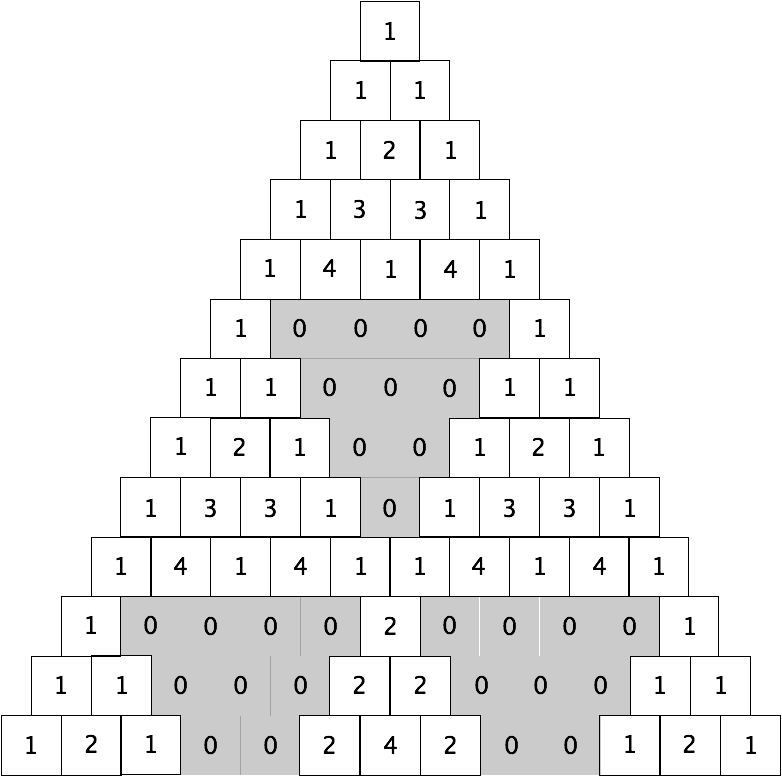
\includegraphics[scale=0.4]{PascalTrianglePrimes}
%        \caption{Regular patterns modulo $5$.}
%        \label{fig:modularPasc-Triangle}
%\end{center}
%\end{figure}
a wondrous transformation happens.  The first $m$ levels of the triangle get replicated endlessly, with an inverted $(m-1)$-level triangle whose entries are all $0$.  (In the figure, the inverted triangle of $0$s is depicted in gray.)  The original triangle has been transformed into a fractal-like repetitive structure whose pattern of repetitions is dictated by the parameter $m$.

\medskip

{\em Prove that the described transformation occurs.}

\smallskip

The $\oplus$ we have assigned to this problem reflects the challenge of figuring out how the various parameters that determine the triangle get transformed by the ``folding".

\item
{\bf A link between perfect numbers and triangular numbers}

{\sc Lesson:} Practice with nonelementary mathematical concepts

\smallskip

Proposition~\ref{thm:MP-PN} (Section~\ref{sec:MP+PN}) tells us that, for every Mersenne prime $2^p-1$, the integer is $2^{p-1} \times (2^p-1)$ is a perfect number.  Let us denote that number by $PN_p$.  A small calculation verifies that both
\[ PN_2 \ = \ 6 \ \ \ \ \ \mbox{ and } \ \ \ \ \ PN_3 \ = \ 28 \]
are triangular numbers, in addition to being perfect; to wit, $6 =\Delta_3$ and $28=\Delta_7$.  This is not a coincidence!

\smallskip

{\em Prove the following result.}

\begin{prop}
For every Mersenne prime $2^p-1$, we have
\[ PN_p \ = \  \Delta_{2^p-1}. \]
\end{prop}

\medskip

{\em Hint:} Explore the defining expression $\Delta_{n} = {1 \over 2} n(n+1)$ for the case $n = 2^{p-1}$. 

%$\Delta_{2^\alpha-1} = \frac{(2^\alpha-1)(2^\alpha-1+1)}{2} = \frac{(2^\alpha-1)(2^\alpha)}{2} = (2^\alpha-1)2^{\alpha-1}$

\item
{\bf Divisibility among integers: via the Fundamental Theorem of Arithmetic}

{\sc Lesson:} Understand the vestiges of divisibility that do exist within the integers

  \begin{enumerate}
  \item
{\bf Cancellation in integer multiplication}

{\sc Lesson:} An exercise in applying the Fundamental Theorem of Arithmetic

\smallskip

\index{cancellation in integer multiplication}

We noted after Proposition~\ref{thm:AR-EX-mult-inv}.b that integers lack multiplicative inverses.  The notion of {\it cancellation} that we describe now can be viewed as a rudimentary form of multiplicative inverses for integers.

\smallskip

{\em Prove the following result.}

\begin{prop}
\label{thm:NUM2-EX-CXL}
Let $m$, $n$, and $p$ be three integers that exceed $1$ (i.e., $m>1$, $n>1$, and $p >1$).  If $m \cdot n = m \times p$, then $n = p$.
\end{prop}

The Fundamental Theorem of Arithmetic yields a particularly charming proof of Proposition~\ref{thm:NUM2-EX-CXL}.

  \item
{\bf The sieve of Eratosthenes and its implications}

{\sc Lessons:} Understand many properties of the integers via the ``sieve"

\index{Eratosthenes of Cyrene}
\index{sieve of Eratosthenes}

\smallskip

The 3rd century BCE Greek polymath Eratosthenes of Cyrene is widely credited with a conceptual algorithm---{\it the sieve}---which identifies the prime factors of integers.  This exercise studies the algorithm and some applications.

\medskip

We formulate the sieve as a regimen for labeling integers with their prime factors.  For simplicity, we use the label $\lambda_p$ to identify integers which are multiples of prime $p$.

\medskip

We begin with the linear array of positive integers:

$\begin{array}{c|c|c|c|c|c|c|c|c|c|c|c|c}
1 & 2 & 3 & 4 & 5 & 6 & 7 & 8 & 9 & 10 & 11 & 12 & 13
\end{array}$ \ldots

\medskip

We label the multiples of $2$ (i.e., the even numbers):

$\begin{array}{c|c|c|c|c|c|c|c|c|c|c|c|c}
1 & 2 & 3 & 4 & 5 & 6 & 7 & 8 & 9 & 10 & 11 & 12 & 13 \\
 & \lambda_2 & & \lambda_2 & & \lambda_2 & & \lambda_2 & & \lambda_2 & & \lambda_2 &
\end{array}$ \ldots

\medskip

We label the multiples of $3$:

$\begin{array}{c|c|c|c|c|c|c|c|c|c|c|c|c}
1 & 2 & 3 & 4 & 5 & 6 & 7 & 8 & 9 & 10 & 11 & 12 & 13 \\
 & \lambda_2 & & \lambda_2 & & \lambda_2 & & \lambda_2 & & \lambda_2 & & \lambda_2 & \\
 & & \lambda_3 & &  & \lambda_3 & & & \lambda_3 & & & \lambda_3 &
\end{array}$ \ldots

\medskip

We label the multiples of $5$:

$\begin{array}{c|c|c|c|c|c|c|c|c|c|c|c|c}
1 & 2 & 3 & 4 & 5 & 6 & 7 & 8 & 9 & 10 & 11 & 12 & 13 \\
 & \lambda_2 & & \lambda_2 & & \lambda_2 & & \lambda_2 & & \lambda_2 & & \lambda_2 & \\
 & & \lambda_3 & &  & \lambda_3 & & & \lambda_3 & & & \lambda_3 & \\
 & & & & \lambda_5 & & & & & \lambda_5 & & & 
\end{array}$ \ldots

\bigskip

The sieve affords one a wonderful perspective for perceiving the patterns that drive mathematical insights.  Here are a few results for you to prove, which are suggested by a perusal of the sieve.

\smallskip

{\em Prove the following results.}
     \begin{enumerate}
     \item
\begin{prop}
Every integer $n>1$ is divisible by at least one prime number.
\end{prop}

     \item
\begin{prop}
Every sequence $k+1, \ldots, k+p$ of $p$ integers contains a multiple of $p$.
\end{prop}

      \item $\oplus$
\begin{prop}
Every product of four consecutive integers, $(k+1) \cdot (k+2) \cdot (k+3) \cdot (k+4)$ is divisible by $4$.
\end{prop}

\smallskip

{\em Hint}:  Look at the {\em multiplicity} with which a given prime divides a given number, particularly within the context of the spacings of the divisibilities---e.g., every even number that is $2 \times$ an odd number is followed by an even number that is $2 \times$ an even number.  These are the ``second-order" insights from the sieve.

\smallskip

{\em Can you come up with extensions of this exercise to other divisors?}

\item
$\oplus$
The sieve affords us an alternative proof that there are infinitely many primes, particularly via the alternative version that is due to Leonhard Euler.  In this version of the sieve, each prime and all of its multiples are removed from the sieve as soon as their existence is acknowledged.  Our earlier construction of Eratosthenes's version of the sieve now becomes:

\index{Euler, Leonhard}
\index{sieve of Euler}

\medskip

$\begin{array}{|l||c|c|c|c|c|c|c|c|c|c|c|c|c|c|}
\hline
\mbox{Initial array:} &
1 & 2 & 3 & 4 & 5 & 6 & 7 & 8 & 9 & 10 & 11 & 12 & 13 & \cdots \\
\mbox{after prime $2$ is processed:} &
1 &  & 3 &  & 5 &  & 7 &  & 9 &  & 11 &  & 13 & \cdots \\
\mbox{after primes $2, 3$ are processed:} &
1 &  &  &  & 5 &  & 7 &  &  &  & 11 &  & 13 & \cdots \\
\mbox{after primes $2, 3, 5$ are processed:} &
1 &  &  &  &  &  & 7 &  &  &  & 11 &  & 13 & \cdots \\
\hspace*{.8in} \vdots  &
 &  &  &  &  &  & \vdots &  &  &  &  &  &  & \\
\hline
\end{array}$


\bigskip

{\em Use Euler's sieve to prove that there are infinitely many primes.}

\medskip

{\em Hint:} If there were only finitely many primes, then at some (finite) stage in processing the sieve, the list of integers would be reduced to the single integer $1$.
     \end{enumerate}
  \end{enumerate}

  \item
$\oplus$
{\bf The ``density"  of divisible pairs of numbers}

{\sc Lesson:} Employing a pigeonhole argument while reasoning about divisibility

\smallskip

{\em Prove that the following assertion is true for every positive integer $n$.}

\begin{prop}
For every positive integer $n$:  If you remove {\em any} $n+1$ integers from the set $S = \{ 1, 2, \ldots, 2n\}$, then the set of removed integers contains at least one pair $p$ and $q > p$ such that $p$ divides $q$.
\end{prop}

\index{Erd\"{o}s, Paul}

This problem was a favorite of the renowned 20th-century Hungarian mathematician Paul Erd\"{o}s, who often used it to test students' mathematical talent.

\smallskip

\textit{Hint:}
Use the Pigeonhole Principle to classify pairs $(p, q > p)$ with respect to divisibility.


\item
{\bf Divisibility and numerals}

{\sc Lessons:} Reinforce understanding of interplay among numbers, numerals, and geometric summations

   \begin{enumerate}
   \item
{\bf On generating numerals from numbers}

{\sc Lesson:} Understanding the importance of Euclidian division

\smallskip

{\em Prove the following assertion.}

\begin{prop}
The successive {\em remainders} from repeated Euclidian divisions of an integer $n$ by a number-base $b$ are the successive digits of the base-$b$ numeral for $n$, from the lowest-order digit to the highest.
\end{prop}

\smallskip

In other words, if the base-$b$ numeral for $n$ is the string
\[ \delta_m \delta_{m-1}  \cdots \delta_1 \delta_0 \]
then the successive remainders are, in order, $\delta_0$, $\delta_1$, \ldots, $\delta_{m-1}$,
$\delta_m$.

   \item
{\bf When is integer $n$ divisible by $9$?}

{\sc Lesson:} Enhance appreciation of positional numerals' grounding in geometric summations

\smallskip

{\em Prove the following assertion.}

\begin{prop}
An integer $n$ is divisible by an integer $m$ if, and only if, $m$ divides the sum of the digits in the base-$(m+1)$ numeral for $n$.
\end{prop}

\smallskip

The most familiar instance of this result states:

{\it An integer $n$ is divisible by $9$ if, and only if, the sum of the digits of $n$'s base-$10$ numeral is divisible by $9$.}

\smallskip

It is important to appreciate that this is not just a party game: It is a basic consequence of the definition of positional number representation.

   \end{enumerate}

\item
{\bf Divisibility under modular arithmetic}

{\sc Lesson:} Enhance ability to reason about modular arithmetic

\smallskip

{\em Prove that the set $\N_q$ is {\em never} closed under the operation of division when the modulus $q$ is composite.}

\item
{\bf The set $\Q$ of rational numbers is countable}

{\sc Lesson:} Practice proving simple properties of highly structured infinite sets.

\smallskip

{\em Prove Proposition~\ref{thm:|Q|=|N|}: $|\Q| \ = \ |\N|$}

\smallskip

{\em Hint}.  You may find it easier to begin with Proposition~\ref{thm:|NxN|=|N|}, which asserts the technically simpler proposition: $|\N \times \N| \ = \ |\N|$.

\end{enumerate}

